\chapter{泊松括號、生成元與角動量}

\lectureoverview{泊松括號不只是簡潔改寫哈密頓方程的工具，也是一種能生成變換的代數運算。與哈密頓量取泊松括號會生成時間演化；與動量取括號會生成平移；與角動量取括號則會生成旋轉。用這種語言來說，對稱性與守恆是同一個零括號的兩種解讀。我們將從諧振子出發發展這個觀念，再利用角動量代數推導陀螺進動，全程不必引入尤拉角。}

\section{沿哈密頓軌跡變化的函數}

設
\[
  F=F(q_1,\ldots,q_n,p_1,\ldots,p_n)
\]
是相空間上的充分可微函數。可以從兩個角度來看它。首先，它為相空間中的每一點指定一個數值。其次，選定一條哈密頓軌跡後，由於點 \((q(t),p(t))\) 隨時間移動，這個函數也就成為時間的函數。沿著該軌跡，
\begin{equation}
  \frac{dF}{dt}
  =
  \sum_i\left(
    \frac{\partial F}{\partial q_i}\dot q_i
    +\frac{\partial F}{\partial p_i}\dot p_i
  \right).
  \label{eq:l8-chain-rule}
\end{equation}
哈密頓方程
\begin{equation}
  \dot q_i=\frac{\partial H}{\partial p_i},
  \qquad
  \dot p_i=-\frac{\partial H}{\partial q_i},
  \label{eq:l8-hamilton-equations}
\end{equation}
可將上式改寫為
\begin{equation}
  \frac{dF}{dt}
  =
  \sum_i\left(
    \frac{\partial F}{\partial q_i}
    \frac{\partial H}{\partial p_i}
    -
    \frac{\partial F}{\partial p_i}
    \frac{\partial H}{\partial q_i}
  \right).
  \label{eq:l8-fdot-expanded}
\end{equation}
右側這個組合在經典力學中屢屢出現，即使其中兩個函數都不是哈密頓量也是如此。因此我們定義
\begin{equation}
  \boxed{
  \{F,G\}
  =
  \sum_i\left(
    \frac{\partial F}{\partial q_i}
    \frac{\partial G}{\partial p_i}
    -
    \frac{\partial F}{\partial p_i}
    \frac{\partial G}{\partial q_i}
  \right).}
  \label{eq:l8-poisson-definition}
\end{equation}
所以，式 ~\eqref{eq:l8-fdot-expanded} 可寫成
\begin{equation}
  \boxed{\dot F=\{F,H\}.}
  \label{eq:l8-time-generator}
\end{equation}

\begin{classroomqa}
  \audiencequestion{若將第二個函數從 \(H\) 換成任意函數 \(G\)，這個括號仍會是 \(F\) 的時間導數嗎？
  \lecturetimestamp{00:05:45--00:06:15}}
  \lecturerresponse{不會。記號推廣時，聽眾注意到了一個重要之處：式 ~\eqref{eq:l8-poisson-definition} 對任意兩個相空間函數定義了 \(\{F,G\}\)，但
  \(\dot F=\{F,G\}\) 只有在 \(G\) 是哈密頓量時才成立。一般的 \(G\) 會生成不同的無窮小變換。}
\end{classroomqa}

將時間的微小變化寫成
\begin{equation}
  \delta_t F=\epsilon\,\{F,H\}.
  \label{eq:l8-small-time-step}
\end{equation}
很有用。這種寫法也預示了後續的內容：時間演化只是由泊松括號生成的一大類變換之一。

\section{括號的代數}

現在可以把括號當作一套獨立的演算來使用。它的規則可由普通微分推出：
\begin{align}
  \{A,B\}&=-\{B,A\}, \label{eq:l8-antisymmetry}\\
  \{A+B,C\}&=\{A,C\}+\{B,C\}, \label{eq:l8-additivity}\\
  \{\lambda A,B\}&=\lambda\{A,B\},
    \quad \lambda\ \text{constant}, \label{eq:l8-scalar-rule}\\
  \{AB,C\}&=A\{B,C\}+\{A,C\}B. \label{eq:l8-leibniz}
\end{align}
這四行依序表達反對稱性、可加性、對常數乘法的線性，以及萊布尼茲法則。經典相空間函數的乘法是可交換的，因此最後一行中的普通因子 \(A\) 與 \(B\) 放置次序無關緊要。量子力學中的算符則不再如此。反對稱性也表示
\begin{equation}
  \{A,A\}=0.
  \label{eq:l8-self-bracket}
\end{equation}

正則座標的基本括號為
\begin{equation}
  \boxed{
  \{q_i,q_j\}=0,\qquad
  \{p_i,p_j\}=0,\qquad
  \{q_i,p_j\}=\delta_{ij}.}
  \label{eq:l8-canonical-brackets}
\end{equation}
任何只依賴 \(q_i\) 的函數，與任何只依賴 \(q_i\) 的函數取括號都為零；只依賴 \(p_i\) 的函數也有類似性質。只有正則座標與其共軛動量相遇時，括號才可能不為零。式 ~\eqref{eq:l8-canonical-brackets} 中的克羅內克 {\proseunicodefont δ} 表示只有指標相同時才會相遇。

\subsection{以諧振子作為檢驗}

考慮
\begin{equation}
  H=\frac{p^2}{2m}+\frac{kq^2}{2}.
  \label{eq:l8-oscillator-hamiltonian}
\end{equation}
現在我們刻意只使用括號規則和式 ~\eqref{eq:l8-time-generator}。首先，
\begin{align}
  \dot q
  &=\{q,H\}\\
  &=\frac{1}{2m}\{q,p^2\}\\
  &=\frac{1}{2m}\left(p\{q,p\}+\{q,p\}p\right)\\
  &=\frac{p}{m}.
  \label{eq:l8-qdot-oscillator}
\end{align}
勢能項會消失，因為 \(\{q,q^2\}=0\)。同樣地，
\begin{align}
  \dot p
  &=\{p,H\}\\
  &=\frac{k}{2}\{p,q^2\}\\
  &=\frac{k}{2}\left(q\{p,q\}+\{p,q\}q\right)\\
  &=-kq.
  \label{eq:l8-pdot-oscillator}
\end{align}
這個負號正是反對稱性 \(\{p,q\}=-\{q,p\}=-1\) 所致。合併這兩個一階方程，得到
\begin{equation}
  m\ddot q=-kq.
  \label{eq:l8-hooke-equation}
\end{equation}

\begin{figure}[htbp]
  \centering
  
\includegraphics[width=0.82\textwidth]{lecture_08_figure_01.png}
  \caption{諧振子的哈密頓量，以及分別導出 \(\dot q=p/m\) 與 \(\dot p=-kq\) 的括號計算。}
  \lectureframe{00:23:20}
\end{figure}

計算過程中，全班試著找出一個表示 \emph{取泊松括號} 的動詞，暫時選定了 \emph{泊松化}。這個玩笑點出觀點上的真正轉變：掌握代數規則後，就能直接運用它，不必每次都從定義重新推導結果。

\begin{classroomqa}
  \audiencequestion{這種數學結構是群，還是代數？它有反元素嗎？\lecturetimestamp{00:23:48--00:24:16}}
  \lecturerresponse{它不是群：括號運算不具備群所需的單位元與反元素。相空間函數構成一個泊松代數：它們具有普通的交換乘法與加法，並配有滿足萊布尼茲法則的反對稱括號。還需要另一個恆等式，也就是雅可比恆等式，才能符合一般的抽象定義；本講不會進一步推導它。}
\end{classroomqa}

\begin{classroomqa}
  \audiencequestion{泊松括號與量子對易子有什麼關聯？\lecturetimestamp{00:24:18--00:25:00}}
  \lecturerresponse{本講只先略作介紹。過渡到量子力學時，經典括號在概略上會以
  \[
    \{A,B\}_{\mathrm{PB}}
    \longleftrightarrow
    \frac{1}{i\hbar}[\widehat A,\widehat B].
  \]
  取代。不過，這種對應關係須附帶算符排序與量子化方面的條件；這裡不會把它當作定理使用。}
\end{classroomqa}

對諧振子而言，泊松括號只是重新推導出哈密頓方程。當生成元是守恆量而非 \(H\) 時，這套方法真正的簡便之處才會顯現。

\section{從旋轉對稱性導出角動量}

回想本課程前面用過的諾特構造之無窮小形式。若連續對稱性使座標產生變化
\begin{equation}
  \delta q_i=\epsilon F_i(q),
  \label{eq:l8-noether-variation}
\end{equation}
那麼，在此處討論的情況下，相應的守恆量為
\begin{equation}
  G=\sum_i p_iF_i(q).
  \label{eq:l8-noether-charge}
\end{equation}
整體因子 \(\epsilon\) 可以省略：守恆量乘上一個固定數，不會改變守恆定律。

取一個粒子，讓它繞 \(z\) 軸作無窮小旋轉。按照本講採用的方向約定，
\begin{equation}
  \delta x=-\epsilon y,\qquad
  \delta y=\epsilon x,\qquad
  \delta z=0.
  \label{eq:l8-z-rotation}
\end{equation}
式 ~\eqref{eq:l8-noether-charge} 給出
\begin{equation}
  L_z=-p_xy+p_yx=xp_y-yp_x.
  \label{eq:l8-lz}
\end{equation}
循環置換 \(x\)、\(y\) 與 \(z\)，可得
\begin{equation}
  \boxed{\begin{aligned}
    L_x&=yp_z-zp_y,\\
    L_y&=zp_x-xp_z,\\
    L_z&=xp_y-yp_x.
  \end{aligned}}
  \label{eq:l8-angular-components}
\end{equation}
這些就是 \begin{equation}
  \boldsymbol L=\boldsymbol r\times\boldsymbol p.
  \label{eq:l8-cross-product}
\end{equation} 的分量。

\begin{figure}[htbp]
  \centering
  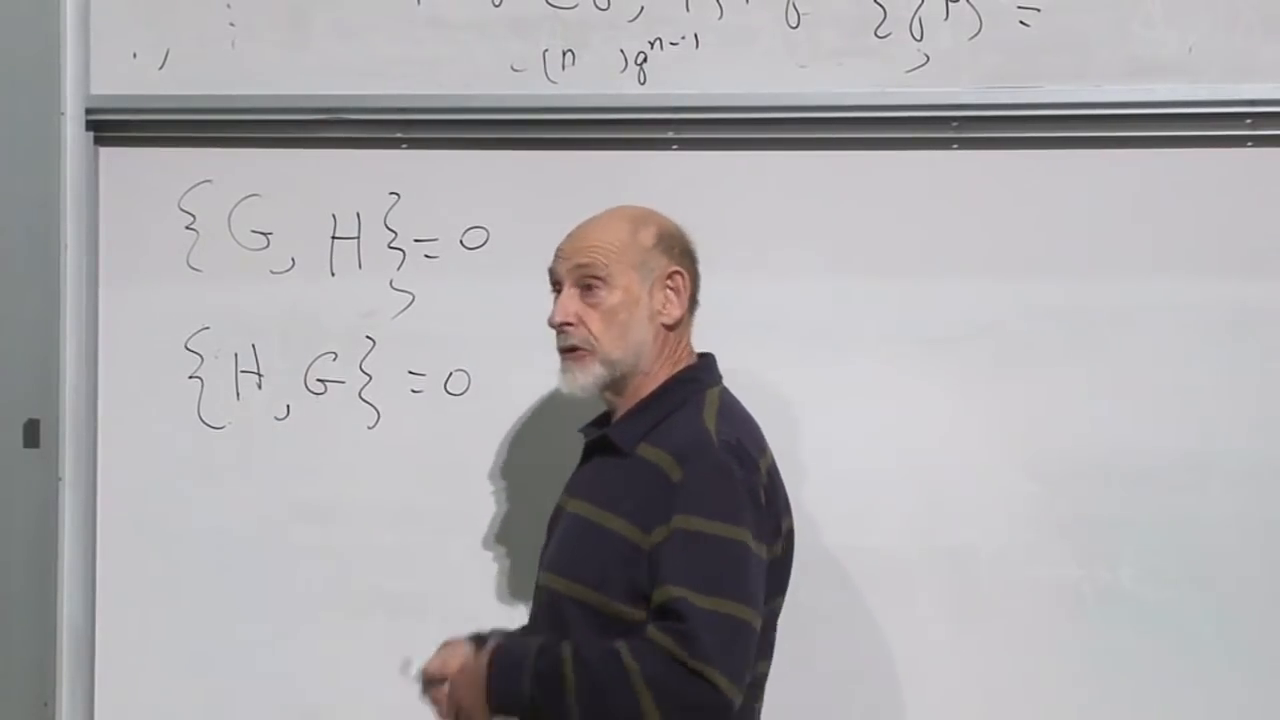
\includegraphics[width=0.82\textwidth]{lecture_08_figure_02.png}
  \caption{角動量的三個笛卡兒分量及其簡潔的叉積表示式。}
  \lectureframe{00:34:00}
\end{figure}

繞任意單位向量 \(\boldsymbol n\) 的旋轉，其生成元為
\begin{equation}
  L_{\boldsymbol n}=\boldsymbol n\cdot\boldsymbol L.
  \label{eq:l8-arbitrary-axis}
\end{equation}
對孤立且具旋轉不變性的系統，角動量的三個分量都守恆。若系統只在繞某一軸旋轉時仍具對稱性，則只有沿該軸的分量必定守恆。

\section{角動量生成旋轉}

我們先不急著求解旋轉動力學問題，而來看看 \(L_z\) 在取括號後會如何作用。利用式 ~\eqref{eq:l8-lz}，
\begin{align}
  \{x,L_z\}
  &=\{x,xp_y-yp_x\}
   =-y\{x,p_x\}
   =-y,\\
  \{y,L_z\}
  &=\{y,xp_y-yp_x\}
   =x\{y,p_y\}
   =x,\\
  \{z,L_z\}&=0.
  \label{eq:l8-position-rotation-brackets}
\end{align}
所得結果恰好就是式 ~\eqref{eq:l8-z-rotation} 中的係數。

\begin{figure}[htbp]
  \centering
  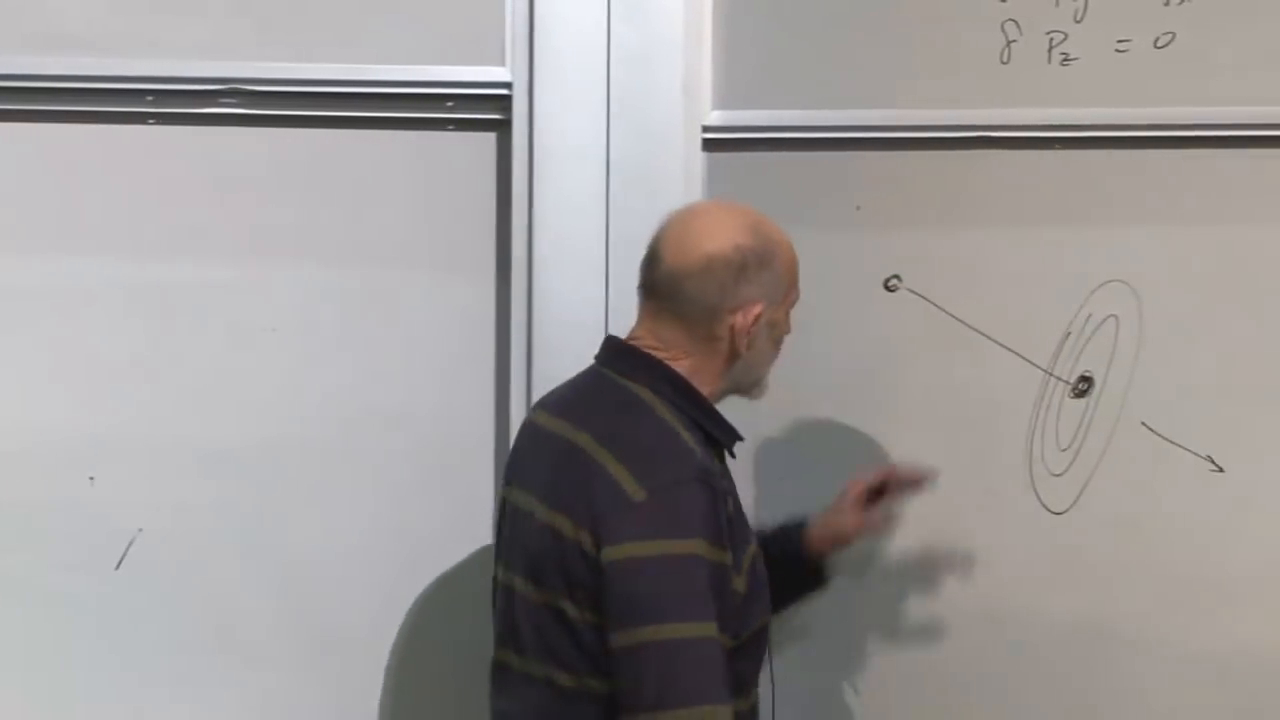
\includegraphics[width=0.82\textwidth]{lecture_08_figure_03.png}
  \caption{座標與 \(L_z\) 的括號：取括號會重現 \((x,y,z)\) 的無窮小旋轉。}
  \lectureframe{00:38:41}
\end{figure}

動量也是向量，同樣的計算得到
\begin{equation}
  \begin{aligned}
    \{p_x,L_z\}&=-p_y,\\
    \{p_y,L_z\}&=p_x,\\
    \{p_z,L_z\}&=0.
  \end{aligned}
  \label{eq:l8-momentum-rotation-brackets}
\end{equation}

\begin{figure}[htbp]
  \centering
  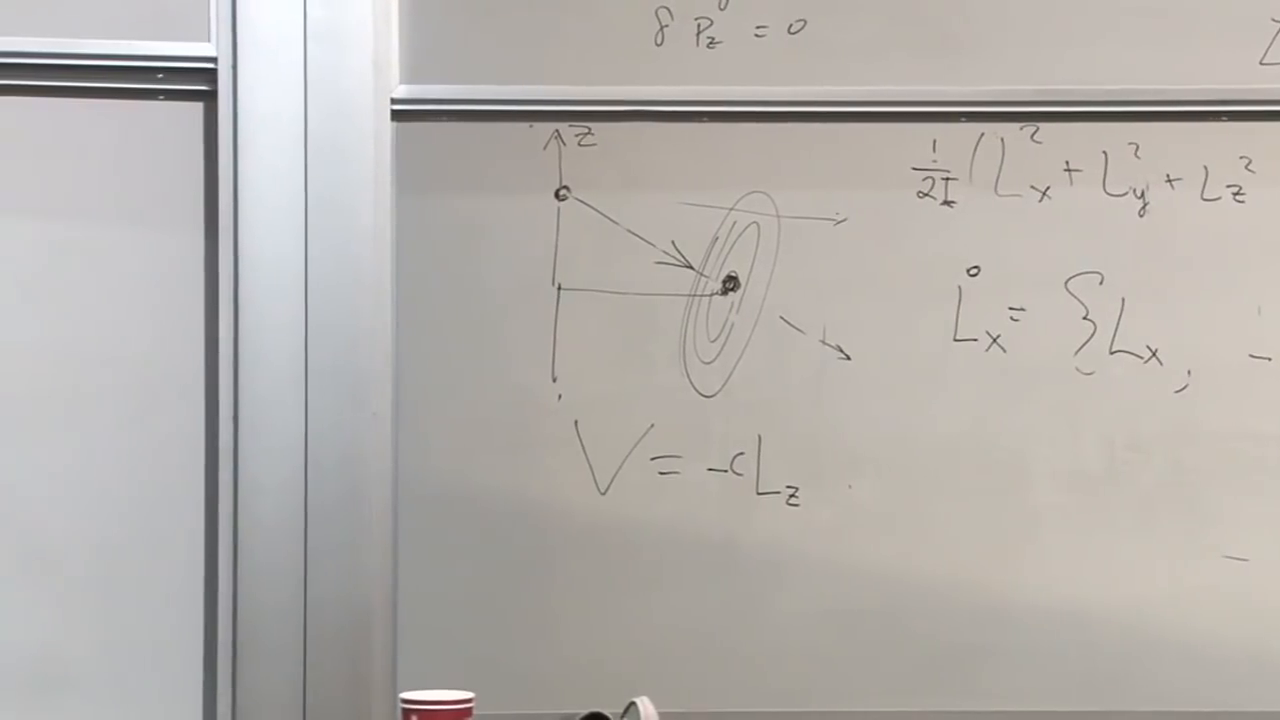
\includegraphics[width=0.82\textwidth]{lecture_08_figure_04.png}
  \caption{在由 \(L_z\) 生成的旋轉下，位置向量與動量向量依照相同的向量變換形式變化。}
  \lectureframe{00:42:08}
\end{figure}

因此，一般的哈密頓表述為
\begin{equation}
  \boxed{\delta_G A=\epsilon\{A,G\}.}
  \label{eq:l8-generator-rule}
\end{equation}
每個相空間函數 \(G\) 都會定義一個這樣的無窮小正則變換。若 \(G=L_z\)，這個變換就是旋轉；若 \(G=H\)，就是時間上的一小步。

\begin{classroomqa}
  \audiencequestion{本講有時談到旋轉系統，有時談到旋轉座標。括號方程採用哪一種約定？\lecturetimestamp{00:28:22--00:29:35}}
  \lecturerresponse{式 ~\eqref{eq:l8-z-rotation} 確立了約定：這裡採用的是無窮小主動旋轉 \((x,y)\mapsto(x-\epsilon y,y+\epsilon x)\)。若被動旋轉座標軸，符號則相反。約定一旦確立，括號公式便沒有歧義。}
\end{classroomqa}

\section{動量生成平移}

沿一個座標方向的平移為
\begin{equation}
  \delta q=\epsilon.
  \label{eq:l8-q-translation}
\end{equation}
在式 ~\eqref{eq:l8-noether-variation} 中，\(F(q)=1\)，因此相應的守恆量是 \(p\)。生成元的說法預測
\begin{equation}
  \{f(q),p\}=\frac{df}{dq}.
  \label{eq:l8-translation-derivative}
\end{equation}
本講先以歸納法證明這個結果適用於冪。基底情況為 \(\{q,p\}=1\)。假設
\begin{equation}
  \{q^{n-1},p\}=(n-1)q^{n-2}.
  \label{eq:l8-induction-hypothesis}
\end{equation}
那麼，根據乘積法則，
\begin{align}
  \{q^n,p\}
  &=\{q\,q^{n-1},p\}\\
  &=q\{q^{n-1},p\}+\{q,p\}q^{n-1}\\
  &=(n-1)q^{n-1}+q^{n-1}\\
  &=nq^{n-1}.
  \label{eq:l8-power-translation}
\end{align}
利用線性性，結果可推廣至多項式與收斂的冪級數表示。更直接地，從括號的定義可得，對每個可微函數 \(f(q)\)，式 ~\eqref{eq:l8-translation-derivative} 都成立：
\begin{equation}
  \{f(q),p\}
  =
  \frac{\partial f}{\partial q}
  \frac{\partial p}{\partial p}
  =f'(q).
\end{equation}

\begin{figure}[htbp]
  \centering
  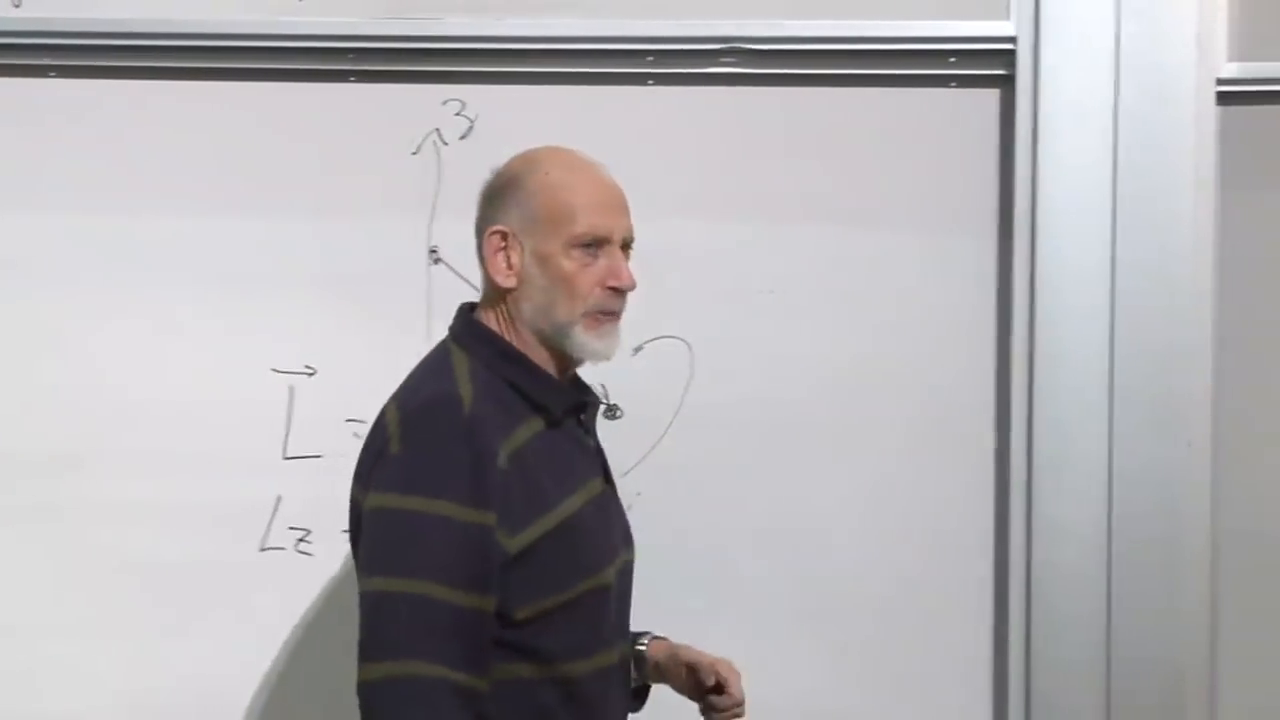
\includegraphics[width=0.82\textwidth]{lecture_08_figure_05.png}
  \caption{歸納證明後得到的平移結果：\(\{F(q),p\}=dF/dq\)。}
  \lectureframe{00:53:18}
\end{figure}

我們已經看到同一個觀念的三種形式：
\begin{center}
  \begin{tabular}{@{}>{\raggedright\arraybackslash}p{0.37\textwidth}
                      >{\raggedright\arraybackslash}p{0.55\textwidth}@{}}
    \toprule
    生成元與變換&無窮小作用\\
    \midrule
    \(H\)，時間平移& \(\delta_tA=\epsilon\{A,H\}\)\\
    \(p_i\)，空間平移& \(\delta A=\epsilon\{A,p_i\}\)\\
    \(L_i\)，旋轉& \(\delta A=\epsilon\{A,L_i\}\)\\
    \bottomrule
  \end{tabular}
\end{center}
與連續對稱性相應的守恆量，同時也是該對稱性的生成元。

\section{一個括號，兩種解讀}

設 \(G(q,p)\) 是候選生成元。若它是守恆量且不顯含時間，則
\begin{equation}
  \dot G=\{G,H\}=0.
  \label{eq:l8-g-conserved}
\end{equation}
由反對稱性可得
\begin{equation}
  \{H,G\}=0.
  \label{eq:l8-h-invariant}
\end{equation}
這兩個方程在數學上等價，但物理解讀不同：
\begin{itemize}
  \item \(\{G,H\}=0\) 表示 \(G\) 在由 \(H\) 生成的時間演化下不變。
  \item \(\{H,G\}=0\) 表示 \(H\) 在由 \(G\) 生成的變換下不變。
\end{itemize}
前者是守恆定律；後者是哈密頓量的對稱性。諾特定理所揭示的關聯，就濃縮在這個零值之中。

\begin{figure}[htbp]
  \centering
  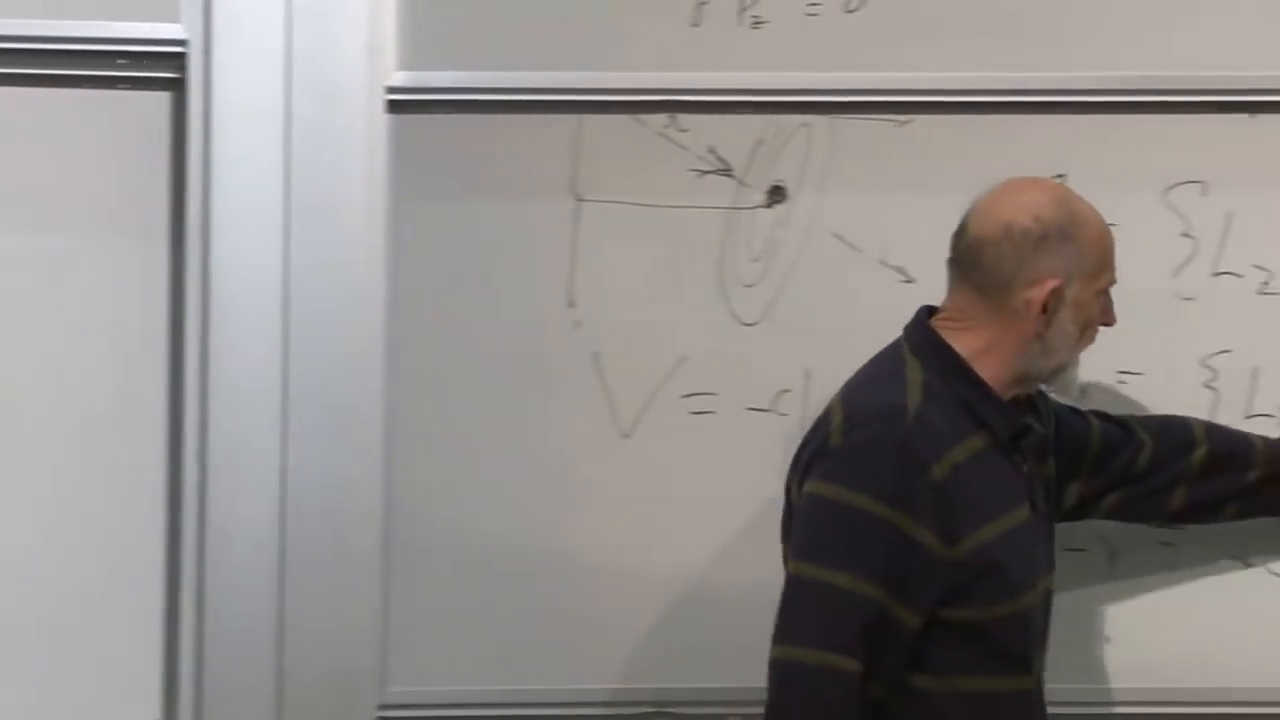
\includegraphics[width=0.82\textwidth]{lecture_08_figure_06.png}
  \caption{同一個零括號的兩種排列：\(G\) 守恆，以及 \(H\) 在由 \(G\) 生成的變換下保持不變。}
  \lectureframe{01:03:05}
\end{figure}

\begin{classroomqa}
  \audiencequestion{若已知某個守恆量，是否總能找出相應的對稱性？\lecturetimestamp{01:01:42--01:02:15}}
  \lecturerresponse{在這個哈密頓力學框架內，可以。將每個相空間變數與 \(G\) 取括號，所得的一組結果 \(\delta_GA=\epsilon\{A,G\}\) 會告訴我們這些變數如何變換。例如，與 \(L_z\) 取括號會顯示出旋轉，即使事先並不知道這種解讀。更進階的情況可能涉及整體性與邊界上的細節；此處使用的是局部的無窮小敘述。}
\end{classroomqa}

\begin{classroomqa}
  \audiencequestion{這些括號方程能告訴我們，究竟是哪種物理運動造成守恆定律嗎？
  \lecturetimestamp{00:56:01--00:58:13}}
  \lecturerresponse{不能。它們指出的是對稱變換，而不是實際軌跡。\(L_z\) 守恆表示系統具有旋轉對稱性，但不代表粒子沿圓周運動。實際的時間演化由 \(H\) 生成；與其他生成元取括號，則描述相空間中另一個方向的變換。}
\end{classroomqa}

\begin{classroomqa}
  \audiencequestion{有沒有不預先假設守恆的一般變換敘述？\lecturetimestamp{01:02:40--01:04:45}}
  \lecturerresponse{有。式 ~\eqref{eq:l8-generator-rule} 對每個函數 \(G\) 都定義了無窮小變換，不論它是否守恆。只有在哈密頓量保持不變時，這個變換才是對稱性：\(\{H,G\}=0\)。反過來讀取同一條件，就表示 \(G\) 是守恆量。}
\end{classroomqa}

\section{角動量代數}

接下來的計算讓我們在處理每個旋轉問題時，不必再逐一追蹤粒子座標。先從
\[
  L_x=yp_z-zp_y,\qquad
  L_z=xp_y-yp_x.
\]
開始。在 \(\{L_x,L_z\}\) 中，大多數交叉項都會消失，因為它們的指標並未形成正則共軛對。留下的縮併項給出
\begin{align}
  \{L_x,L_z\}
  &=\{yp_z-zp_y,xp_y-yp_x\}\\
  &=xp_z-zp_x\\
  &=-L_y.
  \label{eq:l8-lx-lz}
\end{align}
交換括號內兩項的次序，負號便消失。依序輪換座標，可得
\begin{equation}
  \boxed{\begin{aligned}
    \{L_x,L_y\}&=L_z,\\
    \{L_y,L_z\}&=L_x,\\
    \{L_z,L_x\}&=L_y.
  \end{aligned}}
  \label{eq:l8-angular-algebra}
\end{equation}
用指標表示則為
\begin{equation}
  \{L_i,L_j\}=\varepsilon_{ijk}L_k.
  \label{eq:l8-angular-algebra-index}
\end{equation}

\begin{figure}[htbp]
  \centering
  \includegraphics[width=0.82\textwidth]{lecture_08_figure_07.png}
  \caption{三個角動量分量的循環泊松括號代數。}
  \lectureframe{01:10:52}
\end{figure}

這個結果其實也可以預見。既然 \(\boldsymbol L\) 是向量，將它的 \(x\) 分量與 \(L_z\) 取括號，必定會得到該分量在繞 \(z\) 軸旋轉時的無窮小變化，也就是 \(-L_y\)。明確計算驗證了這個幾何論證。這些方程也是量子角動量對易關係的經典前身。

\section{快速旋轉的陀螺}

作為應用，考慮一個陀螺：飛輪快速旋轉，其中心與支點相距 \(R\)。令 \(\boldsymbol r\) 表示從支點指向輪心的向量。飛輪繞軸高速自轉，因此主要角動量保持與該方向平行。在本講採用的近似下，
\begin{equation}
  \boldsymbol L=\ell\,\boldsymbol r,
  \qquad
  L_z=\ell z,
  \label{eq:l8-L-parallel-r}
\end{equation}
其中 \(\ell=L/R\) 視為常數。起初先忽略與章動或轉軸運動相關的較小角動量。

\begin{figure}[htbp]
  \centering
  \begin{tikzpicture}[scale=0.95,>=Latex]
    \coordinate (P) at (0,3.2);
    \coordinate (C) at (3.7,1.55);
    \draw[->] (0,-0.2) -- (0,4.35) node[above] {\(z\)};
    \fill (P) circle (1.7pt) node[left] {pivot};
    \draw[very thick,->] (P) -- (C)
      node[midway,above right] {\(\boldsymbol r\parallel\boldsymbol L\)};
    \fill (C) circle (1.7pt);
    \draw[dashed] (P) -- (0,1.55);
    \draw[dashed] (0,1.55) -- (C);
    \node[left] at (0,1.55) {\(z\)};
    \begin{scope}[shift={(C)},rotate=-24]
      \draw[very thick] (0,0) ellipse (0.65 and 1.35);
      \draw[thick] (0,0) ellipse (0.42 and 0.9);
    \end{scope}
    \draw[->,thick] (2.15,2.85)
      arc[start angle=140,end angle=35,radius=1.65];
  \end{tikzpicture}
  \caption{快速陀螺近似：支點至輪心的距離固定，主要自轉角動量保持與轉軸及 \(\boldsymbol r\) 平行。}
\end{figure}

\begin{figure}[htbp]
  \centering
  \includegraphics[width=0.82\textwidth]{lecture_08_figure_08.png}
  \caption{黑板上的飛輪示意圖，並列出 \(H_{\rm rot}=L^2/(2I)\)；其中的抵消說明了無力矩時 \(\boldsymbol L\) 守恆。}
  \lectureframe{01:18:54}
\end{figure}

\subsection{無重力時：為何每個分量都保持不變}

對簡化的軸對稱轉子而言，
\begin{equation}
  H_{\mathrm{rot}}
  =\frac{1}{2I}
  \left(L_x^2+L_y^2+L_z^2\right)
  =\frac{L^2}{2I}.
  \label{eq:l8-rotational-hamiltonian}
\end{equation}
係數應為 \(1/(2I)\)，而非 \(I/2\)；講者在黑板上寫錯後隨即更正。利用式 ~\eqref{eq:l8-angular-algebra}，
\begin{align}
  \dot L_x
  &=\{L_x,H_{\mathrm{rot}}\}\\
  &=\frac{1}{2I}\left(
    2L_y\{L_x,L_y\}
    +2L_z\{L_x,L_z\}
  \right)\\
  &=\frac{1}{I}\left(L_yL_z-L_zL_y\right)=0.
  \label{eq:l8-free-lx}
\end{align}
循環置換各分量，可得
\begin{equation}
  \dot L_x=\dot L_y=\dot L_z=0.
  \label{eq:l8-free-angular-momentum}
\end{equation}
純量 \(L^2\) 與每個分量 \(L_i\) 的括號都為零；依這套代數的術語，它是卡西米爾量。因此，無力矩作用的陀螺，其角動量的大小與方向都保持不變。

\begin{classroomqa}
  \audiencequestion{這裡的轉動慣量只是純量嗎？
  \lecturetimestamp{01:14:23--01:15:05}}
  \lecturerresponse{對這個簡化模型來說，是的。它描述飛輪繞自轉軸的質量分布。一般剛體則有轉動慣量張量，而在主軸座標系中，轉動哈密頓量為 \(\sum_i L_i^2/(2I_i)\)。本講選用較簡單的高速對稱轉子，目的是展示泊松括號方法，而非完整探討剛體動力學。}
\end{classroomqa}

\subsection{重力與位能的符號}

令垂直座標 \(z\) 向上為正，並將支點設在原點。輪心的重力位能為
\begin{equation}
  V=Mgz.
  \label{eq:l8-mgz}
\end{equation}
由於 \(L_z=\ell z\)，
\begin{equation}
  V=cL_z,
  \qquad
  c=\frac{Mg}{\ell}=\frac{MgR}{L}.
  \label{eq:l8-potential-lz}
\end{equation}
當 \(\boldsymbol L\) 的方向與 \(\boldsymbol r\) 平行時，這裡有 \(c>0\)。若飛輪以相反方向自轉，\(\boldsymbol L\) 與 \(\boldsymbol r\) 之間的帶符號比例關係會反轉，相應的帶符號進動頻率也會反轉。

\begin{figure}[htbp]
  \centering
  \includegraphics[width=0.82\textwidth]{lecture_08_figure_09.png}
  \caption{定長幾何所導出的關係：\(\boldsymbol L=\ell\boldsymbol r\) 與 \(L_z=\ell z\)。}
  \lectureframe{01:25:38}
\end{figure}

\begin{figure}[htbp]
  \centering
  \includegraphics[width=0.82\textwidth]{lecture_08_figure_10.png}
  \caption{黑板上的中間推導曾寫成 \(V=-cL_z\)。後來確定 \(z\) 向上為正後，修正了符號：當 \(\boldsymbol L=\ell\boldsymbol r\) 且 \(\ell>0\) 時，一致的結果是 \(V=+cL_z\)。}
  \lectureframe{01:22:43}
\end{figure}

\begin{classroomqa}
  \audiencequestion{為什麼可以用角動量的一個分量取代高度？那條斜線代表轉軸，還是位置向量？
  \lecturetimestamp{01:22:20--01:25:43}}
  \lecturerresponse{那條斜線最好標為 \(\boldsymbol r\)，也就是從固定支點指向輪心的向量。實際轉軸可能沿著這個方向，但計算所用的關係是快速自轉近似 \(\boldsymbol L=\ell\boldsymbol r\)，因此兩者的 \(z\) 分量成正比。課堂討論曾多次更改標記，最後才確立這項區分。}
\end{classroomqa}

\begin{classroomqa}
  \audiencequestion{哪些假設使 \(\ell\) 保持不變？若輪心能沿徑向滑動，會有什麼問題？
  \lecturetimestamp{01:25:43--01:26:38,\allowbreak\ 01:34:22--01:35:00}}
  \lecturerresponse{假設主要自轉角動量遠大於慢速運動所帶來的角動量，並且支點至輪心的距離固定。如此一來，自轉角動量的大小變化不大，而 \(\boldsymbol L\) 會隨 \(\boldsymbol r\) 一起轉動。若輪心能沿徑向滑動，\(z\) 就不再以固定比例係數與 \(L_z\) 成正比，因此簡化哈密頓量 \(V=cL_z\) 將無法描述其運動。}
\end{classroomqa}

\begin{classroomqa}
  \audiencequestion{為什麼黑板上起初寫負號，後來又改成正號？自轉方向有影響嗎？
  \lecturetimestamp{01:27:13--01:28:15,\allowbreak\ 01:33:09--01:33:21}}
  \lecturerresponse{起初的符號是黑板推導中的錯誤，也混入了尚未確定的軸方向約定。一旦定義 \(z\) 向上，位能 \(V=Mgz\) 就隨高度增加。若 \(\boldsymbol L=\ell\boldsymbol r\) 且 \(\ell>0\)，便得到 \(V=+cL_z\)。反轉自轉方向會使帶符號的比例關係與進動方向反轉，但符號不能任意選取。}
\end{classroomqa}

\subsection{由三個簡短方程導出進動}

完整的簡化哈密頓量為
\begin{equation}
  H=
  \frac{1}{2I}\left(L_x^2+L_y^2+L_z^2\right)+cL_z.
  \label{eq:l8-full-gyro-hamiltonian}
\end{equation}
我們已經證明 \(L^2\) 與每個 \(L_i\) 的括號都為零。因此只有線性項有貢獻：
\begin{align}
  \dot L_z&=\{L_z,H\}=0,\\
  \dot L_x&=\{L_x,H\}=c\{L_x,L_z\}=-cL_y,\\
  \dot L_y&=\{L_y,H\}=c\{L_y,L_z\}=cL_x.
  \label{eq:l8-precession-equations}
\end{align}

\begin{figure}[htbp]
  \centering
  \includegraphics[width=0.82\textwidth]{lecture_08_figure_11.png}
  \caption{最後得到的分量方程：\(L_z\) 保持不變，而 \(L_x\) 與 \(L_y\) 彼此轉換。}
  \lectureframe{01:30:35}
\end{figure}

垂直分量與水平分量的大小都保持不變：
\begin{equation}
  \frac{d}{dt}(L_x^2+L_y^2)
  =2L_x(-cL_y)+2L_y(cL_x)=0.
\end{equation}
合併水平分量，得到
\begin{equation}
  L_+=L_x+iL_y,
  \qquad
  \dot L_+=icL_+,
\end{equation}
因此
\begin{equation}
  L_+(t)=L_+(0)e^{ict}.
  \label{eq:l8-precession-solution}
\end{equation}
角動量向量便以角速度 \(|c|=MgR/L\) 繞垂直軸進動。在這個理想化的定常運動中，其傾角保持不變。

\begin{classroomqa}
  \audiencequestion{寫出進動方程時，轉動能項有被忽略嗎？
  \lecturetimestamp{01:35:01--01:35:49}}
  \lecturerresponse{沒有。它包含在完整哈密頓量中，如式 ~\eqref{eq:l8-full-gyro-hamiltonian} 所示。它對 \(\dot L_i\) 的貢獻為零，因為 \(\{L_i,L^2\}=0\)；這項抵消已在無力矩的計算中證明。學生的提問讓這個原本隱含的步驟明確呈現出來。}
\end{classroomqa}

\begin{classroomqa}
  \audiencequestion{等速進動算是一種平衡嗎？受到輕微擾動後會如何？\lecturetimestamp{01:32:38--01:33:08}}
  \lecturerresponse{與其稱為靜態平衡，不如稱為穩態運動或定常運動。輕微擾動通常會引入章動，也就是傾角的振盪。飛輪自轉得非常快時，振盪幅度很小，因此簡化分析只考慮近似等速的進動。}
\end{classroomqa}

\begin{classroomqa}
  \audiencequestion{進動一定需要支架或實際的轉軸嗎？
  \lecturetimestamp{01:31:49--01:32:38,\allowbreak\ 01:33:49--01:35:00}}
  \lecturerresponse{這個力學模型假設支點至輪心的距離固定，因此必須有某種約束提供支撐。更一般的代數結果則是：只要哈密頓量中有一項與角動量的某個分量成正比，同樣的括號代數便會導出進動。角動量的微觀來源不一定是實際裝在轉軸上的輪子。}
\end{classroomqa}

\begin{classroomqa}
  \audiencequestion{這和磁場中的電子自旋或核自旋進動，或行星軌道進動，是同一種現象嗎？
  \lecturetimestamp{01:35:50--01:37:00}}
  \lecturerresponse{磁矩與磁場耦合時，哈密頓量會與自旋的一個分量成正比，因此遵循相同的角動量代數。核自旋進動是核磁共振的基礎。行星軌道近日點的進動則是另一種現象，只是也使用「\emph{進動}」一詞；兩者的計算並不相同。}
\end{classroomqa}

\begin{classroomqa}
  \audiencequestion{側向安裝的陀螺儀，基本上和旋轉陀螺是同一種物體嗎？\lecturetimestamp{01:37:02--01:37:23}}
  \lecturerresponse{是。兩者的差別主要在幾何上的稱呼：自轉軸從支座向側方伸出時，通常稱為陀螺儀；自轉軸接近垂直時，則通常稱為陀螺。它們的角動量與力矩結構相同。}
\end{classroomqa}

\section{這項計算的成果}

整個過程沒有引入尤拉角，也沒有追蹤飛輪各部分的座標。一旦知道 \[
  \{L_i,L_j\}=\varepsilon_{ijk}L_k
\]，便能直接得到所關心變數的方程。這正是本講要展示的威力。諧振子說明泊松括號可以重現熟悉的動力學；角動量則顯示它們的用途遠不止於此：
\begin{itemize}
  \item 守恆量會生成與之相應的無窮小對稱性；
  \item  \(G\) 的守恆與 \(H\) 的不變性，是 \(\{G,H\}=0\) 的兩種解讀；
  \item 可觀測量的代數可以形成封閉系統，讓我們不必回到微觀座標就能求解動力學；
  \item 哈密頓量若與角動量的一個分量成正比，就會產生繞該軸的進動。
\end{itemize}
本講尚未推導一般剛體的完整尤拉方程，但較為聚焦的結論已經完整：選對生成元並運用其泊松代數，就能以極精簡的方式揭示對稱性與運動。